\documentclass[12pt]{article}
\usepackage[ukrainian,shorthands=off]{babel}   % shorthands=off: символ " не активний (потрібно для міток "..." у TikZ всередині \zadtask)
\usepackage{fontspec}
% --- НАЛАШТУВАННЯ ШРИФТІВ ---
% Шрифти Schoolbook-*.otf лежать у корені проєкту. Шлях підбирається автоматично:
% ../ (компіляція з папки теми), ./ (корінь проєкту), ../../ (підпапки теми 28); інакше -- TeX Gyre Schola.
\newcommand{\nmtSchoolbook}[1]{\setmainfont{Schoolbook-Regular.otf}[
    Path = #1,
    BoldFont = Schoolbook-Bold.otf,
    ItalicFont = Schoolbook-Italic.otf,
    BoldItalicFont = Schoolbook-BoldItalic.otf
]}
\IfFileExists{../Schoolbook-Regular.otf}{\nmtSchoolbook{../}}{%
 \IfFileExists{./Schoolbook-Regular.otf}{\nmtSchoolbook{./}}{%
  \IfFileExists{../../Schoolbook-Regular.otf}{\nmtSchoolbook{../../}}{%
   \setmainfont{texgyreschola}[Extension=.otf, UprightFont=*-regular, BoldFont=*-bold, ItalicFont=*-italic, BoldItalicFont=*-bolditalic]}}}
\usepackage[italic]{mathastext}
\usepackage[a4paper,margin=1.8cm,bottom=2cm,top=2cm]{geometry}
\usepackage{amsmath,amssymb}
\usepackage{tikz}
\usepackage{pgfplots}
\pgfplotsset{compat=1.18}
\usepgfplotslibrary{fillbetween}
\usetikzlibrary{calc,patterns,angles,quotes,intersections,babel,3d,shapes.symbols,shapes.geometric,decorations.pathreplacing,shadings,arrows.meta,hobby}
\usepackage{xcolor,array,fancyhdr,enumitem,multicol}
\usepackage{colortbl,multirow,diagbox,needspace}
\usepackage{tcolorbox}
\tcbuselibrary{skins,breakable}
\usepackage[hidelinks]{hyperref}
% водяний знак; щоб зібрати без нього (версія для вчителів), перед \documentclass пишуть \def\nmtnowatermark{}
\ifdefined\nmtnowatermark\else
\usepackage[firstpage=false, text=@pvtr2525, scale=0.6, color=gray!12]{draftwatermark}
\fi

% --- АВТОСТИСКАННЯ: рисунок/сітка, ширша за колонку, масштабується до ширини колонки ---
\newsavebox{\nmtfitbox}
\newenvironment{nmtfit}{\begin{lrbox}{\nmtfitbox}}{\end{lrbox}%
  \ifdim\wd\nmtfitbox>\linewidth \resizebox{\linewidth}{!}{\usebox{\nmtfitbox}}\else\usebox{\nmtfitbox}\fi}
\let\nmtIncludegraphicsOrig\includegraphics
\renewcommand{\includegraphics}[2][]{\begin{nmtfit}\nmtIncludegraphicsOrig[#1]{#2}\end{nmtfit}}


\definecolor{mainGreen}{RGB}{34, 120, 64}
\definecolor{yearOrange}{RGB}{220, 100, 30}
\definecolor{yearcolor}{RGB}{220, 100, 30}
\definecolor{titleBg}{RGB}{225, 240, 220}
\definecolor{instrBg}{RGB}{255, 240, 220}
\definecolor{instrBorder}{RGB}{220, 150, 80}
\definecolor{headerblue}{RGB}{0, 102, 204}   % використовується в рисунках старої бази

\setlength{\parindent}{0pt}
\emergencystretch=1.5em

\pagestyle{fancy}
\fancyhf{}
\renewcommand{\headrulewidth}{0.4pt}
\renewcommand{\footrulewidth}{0.4pt}
\fancyhead[C]{\small\color{gray!80} Варіант № 3}
\fancyhead[R]{\small\color{mainGreen}\textbf{\href{https://t.me/pvtr2525}{@pvtr2525}}}
\fancyfoot[L]{\small\color{gray!80}\href{https://t.me/pvtr2525}{ТГ: @pvtr2525}}
\fancyfoot[C]{\small\color{gray!80}\thepage}
\fancyfoot[R]{\small\color{gray!80}НМТ з математики}

% --- ТАБЛИЦІ ВІДПОВІДЕЙ ---
% ширина клітинки = (ширина рядка - відступи) / 5: на всю сторінку це ~3 см, у minipage поруч із рисунком таблиця стискається
\newlength{\nmtcellw}
\newcommand{\nmtSetCell}{\setlength{\nmtcellw}{\dimexpr(\linewidth-12\tabcolsep-6\arrayrulewidth)/5\relax}}
\newcommand{\answerTable}[5]{%
\par\nopagebreak\vspace{0.15cm}
\noindent\nmtSetCell
\begin{tabular}{|*{5}{>{\centering\arraybackslash}m{\nmtcellw}|}}
\hline
\rule[-0.15cm]{0pt}{0.6cm}\textbf{А} & \rule[-0.15cm]{0pt}{0.6cm}\textbf{Б} & \rule[-0.15cm]{0pt}{0.6cm}\textbf{В} & \rule[-0.15cm]{0pt}{0.6cm}\textbf{Г} & \rule[-0.15cm]{0pt}{0.6cm}\textbf{Д} \\
\hline
\rule[-0.2cm]{0pt}{0.75cm}#1 & \rule[-0.2cm]{0pt}{0.75cm}#2 & \rule[-0.2cm]{0pt}{0.75cm}#3 & \rule[-0.2cm]{0pt}{0.75cm}#4 & \rule[-0.2cm]{0pt}{0.75cm}#5 \\
\hline
\end{tabular}
\par\vspace{0.25cm}
}
\newcommand{\answerTableTall}[5]{%
\par\nopagebreak\vspace{0.15cm}
\noindent\nmtSetCell
\begin{tabular}{|*{5}{>{\centering\arraybackslash}m{\nmtcellw}|}}
\hline
\rule[-0.2cm]{0pt}{0.7cm}\textbf{А} & \rule[-0.2cm]{0pt}{0.7cm}\textbf{Б} & \rule[-0.2cm]{0pt}{0.7cm}\textbf{В} & \rule[-0.2cm]{0pt}{0.7cm}\textbf{Г} & \rule[-0.2cm]{0pt}{0.7cm}\textbf{Д} \\
\hline
\rule[-0.45cm]{0pt}{1.2cm}#1 & \rule[-0.45cm]{0pt}{1.2cm}#2 & \rule[-0.45cm]{0pt}{1.2cm}#3 & \rule[-0.45cm]{0pt}{1.2cm}#4 & \rule[-0.45cm]{0pt}{1.2cm}#5 \\
\hline
\end{tabular}
\par\vspace{0.25cm}
}
\newcommand{\instructionBox}[1]{%
\par\vspace{0.3cm}
\begin{tcolorbox}[colback=instrBg, colframe=instrBorder, boxrule=0.6pt, arc=2pt,
    left=8pt, right=8pt, top=4pt, bottom=4pt]
\centering\small\bfseries #1
\end{tcolorbox}
\par\vspace{0.15cm}
}
\newcommand{\sectionTitle}[1]{%
\par\vspace{0.4cm}
\begin{tcolorbox}[colback=titleBg, colframe=titleBg, boxrule=0pt, arc=8pt,
    halign=center, fontupper=\Large\bfseries\color{mainGreen}]
\hyphenpenalty=10000 \exhyphenpenalty=10000 #1
\end{tcolorbox}
\par\vspace{0.3cm}
}
\newcommand{\task}[2]{\noindent\textbf{#1.}\ \ #2\par\vspace{0.2cm}}
% --- НМТ-СТИЛЬ ПОЛЕ ВІДПОВІДІ ---
\newcommand{\nmtAnswerBox}{%
\par\nopagebreak\vspace{0.2cm}\noindent
Відповідь:\ \
\begin{tabular}{@{}*{4}{|>{\centering\arraybackslash}p{0.8cm}}|@{\hspace{0.1cm}\textbf{,}\hspace{0.1cm}}*{3}{|>{\centering\arraybackslash}p{0.8cm}}|@{}}
\hline
\rule[-0.2cm]{0pt}{0.7cm} & & & & & & \\
\hline
\end{tabular}
\par\vspace{0.3cm}
}
% --- СІТКА ДЛЯ МАТЧИНГУ ---
\newsavebox{\nmtgridbox}
\newcommand{\matchingGrid}{%
    \sbox{\nmtgridbox}{\matchingGridRaw}%
    \ifdim\wd\nmtgridbox>\linewidth \resizebox{\linewidth}{!}{\usebox{\nmtgridbox}}\else\usebox{\nmtgridbox}\fi}
\newcommand{\matchingGridRaw}{%
    \begingroup
    \renewcommand{\arraystretch}{1.15}
    \setlength{\tabcolsep}{4pt}
    \footnotesize
    \begin{tabular}{r|c|c|c|c|c|}
         \multicolumn{1}{c}{} & \multicolumn{1}{c}{\textbf{А}} & \multicolumn{1}{c}{\textbf{Б}} & \multicolumn{1}{c}{\textbf{В}} & \multicolumn{1}{c}{\textbf{Г}} & \multicolumn{1}{c}{\textbf{Д}} \\ \cline{2-6}
         \textbf{1} & \phantom{X} & \phantom{X} & \phantom{X} & \phantom{X} & \phantom{X} \\ \cline{2-6}
         \textbf{2} & & & & & \\ \cline{2-6}
         \textbf{3} & & & & & \\ \cline{2-6}
    \end{tabular}
    \endgroup
}
% --- ДОДАТКОВІ МАКРОСИ ЗБІРНИКА ---
\newcommand{\taskBlock}[1]{%
\par\vspace{0.45cm}
\noindent{\color{mainGreen}\rule{\linewidth}{0.8pt}}\par\vspace{0.12cm}
\noindent{\small\bfseries\color{mainGreen}#1}\par\vspace{0.25cm}
}
\newcounter{zad}
\newcommand{\zadtask}[1]{\stepcounter{zad}\noindent\textbf{\thezad.}\ \ #1\par\nopagebreak\vspace{0.2cm}}
\newcommand{\zadnum}{\stepcounter{zad}\textbf{\thezad.}\ \ }
\newcounter{ans}
\newcommand{\ansitem}[1]{\stepcounter{ans}\noindent\textbf{\theans.}\ #1\par\vspace{0.07cm}}
% мітка року: нерозривна, притиснута праворуч; якщо не вміщається -- праворуч на новому рядку
\newcommand{\nmtyear}[1]{\unskip\nobreak\finalhyphendemerits=0 \hfill\penalty100\hskip1em\hbox{}\nobreak\hfill{\small\color{yearOrange}\mbox{\rule{0pt}{2.3ex}(НМТ~#1)}}}
% --- МАКРОС КОРОТКОГО РОЗВ'ЯЗКУ ---
\newcommand{\solution}[1]{%
\par\vspace{0.12cm}
\begin{tcolorbox}[colback=titleBg!45, colframe=mainGreen!55, boxrule=0.4pt, arc=2pt,
    left=6pt, right=6pt, top=3pt, bottom=3pt, breakable]
\footnotesize\textbf{Короткий розв'язок.}\ #1
\end{tcolorbox}
\par\vspace{0.12cm}
}
% Розв'язки й відповіді (є до завдань НМТ-2026): \showsolutionstrue -- показати, \showsolutionsfalse -- сховати
\newif\ifshowsolutions
\showsolutionsfalse
% --- ЗАГОЛОВКИ З ПУНКТАМИ КЛІКАБЕЛЬНОГО ЗМІСТУ ---
\setcounter{tocdepth}{2}
\newcommand{\chapterTitle}[1]{%
\clearpage\phantomsection\addcontentsline{toc}{section}{#1}%
\sectionTitle{#1}}
\newcommand{\typeTitle}[1]{%
\needspace{6\baselineskip}%
\phantomsection\addcontentsline{toc}{subsection}{\quad #1}%
\par\vspace{0.3cm}
\noindent{\large\bfseries\color{yearOrange}#1}\par\vspace{0.08cm}
\noindent{\color{yearOrange}\rule{\linewidth}{0.4pt}}\par\nopagebreak\vspace{0.2cm}}
\raggedbottom
% усередині одного завдання сторінка не розривається: нерозривний вертикальний проміжок
% і нерозривна межа абзаців (умова ніколи не відділяється від варіантів, рисунка чи сітки)
\newcommand{\nbvspace}[1]{\nopagebreak\vspace{#1}}
\newcommand{\nmtnobreak}{\ifvmode\penalty10000 \fi}
% --- ЄДИНИЙ МАКЕТ ЗАВДАНЬ НА ВІДПОВІДНІСТЬ ---
% мітка в колонці сталої ширини, текст -- у parbox: продовження довгого рядка
% вирівнюється під текстом, а не під міткою; відступ між пунктами однаковий скрізь
\newlength{\nmtMatchLab}\setlength{\nmtMatchLab}{1.6em}
\newlength{\nmtMatchSep}\setlength{\nmtMatchSep}{0.28cm}
\newcommand{\matchHead}[1]{\par\noindent\textit{#1}\par\nopagebreak\vspace{0.2cm}}
\newcommand{\matchItem}[2]{\par\noindent\makebox[\nmtMatchLab][l]{\textbf{#1}}%
\parbox[t]{\dimexpr\linewidth-\nmtMatchLab\relax}{\raggedright #2}\par\nopagebreak\vspace{\nmtMatchSep}}
\newcommand{\ansTheme}[1]{\par\vspace{0.25cm}\noindent{\bfseries\color{mainGreen}#1}\par\vspace{0.12cm}}
\newcommand{\ansType}[1]{\par\vspace{0.1cm}\noindent{\itshape\color{yearOrange}#1}\par\vspace{0.08cm}}

\graphicspath{{../1. Числа. Звичайні та десяткові дроби. Модуль числа/}{../10. Основи планіметрії/}{../11. Трикутники/}{../12. Паралелограм/}{../13. Прямокутник/}{../14. Квадрат/}{../15. Ромб/}{../16. Трапеція/}{../17. Коло, круг і їх елементи/}{../18. Координати і вектори на площині і в просторі. Рівняння кола/}{../19. Лінійні та квадратні нерівності. Системи лінійних нерівностей. Метод інтервалів/}{../2.відсотки, арифметичні задачі, подільність/}{../20. Функція та її властивості/}{../21.  Графіки елементарних функцій, їх побудова графіків функцій та їх перетворення/}{../22. Модульні  рівняння та нерівності/}{../23. Ірраціональні рівняння та нерівності/}{../24. Арифметична прогресія/}{../25. Геометрична прогресія/}{../26. Тригонометричні вирази/}{../27. Тригонометричні рівняння/}{../28. Показникова функція. Показникові рівняння/Показникові рівняння/}{../28. Показникова функція. Показникові рівняння/Показникові функція і вирази/}{../29. Показникові нерівності/}{../3. Степені. Одночлени. стандартний вигляд числа/}{../30. Логарифм. Логарифмічна функція/}{../31. Логарифмічні рівняння/}{../32. Логарифмічні нерівності/}{../33. Похідна/}{../34. Первісна/}{../35. Комбінаторика/}{../36. Теорія ймовірності/}{../37. Статистика/}{../38. Призма. Паралелепіпед. Куб/}{../39. Піраміда/}{../4.Многочлени. ФСМ/}{../40. Циліндр/}{../41. Конус/}{../42. Куля. Сфера/}{../43. Параметри/}{../5. дробові раціональні вирази і перетворення/}{../6. Лінійні рівняння/}{../7. Квадратні корені. Корені вищих степенів. Раціональний степінь/}{../8. квадратні рівняння, і рівняння, що до них зводяться/}{../9. Системи рівнянь/}}

\begin{document}
% макроси бази, потрібні аналогам
% --- сумісність зі старою базою (діє, якщо тема не має власного визначення) ---
\providecommand{\trigStyle}[1]{#1}
\providecommand{\answerTableSmall}[5]{%
\begingroup\setlength{\tabcolsep}{2pt}\small\nmtSetCell
\begin{tabular}{|*{5}{>{\centering\arraybackslash}m{\nmtcellw}|}}
\hline
\rule[-0.2cm]{0pt}{0.6cm}\textbf{А} & \textbf{Б} & \textbf{В} & \textbf{Г} & \textbf{Д} \\
\hline
\rule[-0.4cm]{0pt}{0.9cm}#1 & \rule[-0.4cm]{0pt}{0.9cm}#2 & \rule[-0.4cm]{0pt}{0.9cm}#3 & \rule[-0.4cm]{0pt}{0.9cm}#4 & \rule[-0.4cm]{0pt}{0.9cm}#5 \\
\hline
\end{tabular}\endgroup}
\providecommand{\matchingLayout}[3]{%
    \noindent
    \begin{minipage}[t]{0.36\textwidth}\vspace{0pt}\raggedright
        #1
    \end{minipage}%
    \hfill
    \begin{minipage}[t]{0.43\textwidth}\vspace{0pt}\raggedright
        #2
    \end{minipage}%
    \hfill
    \begin{minipage}[t]{0.19\textwidth}
        \vspace{0pt}
        \begin{flushright}
        #3
        \end{flushright}
    \end{minipage}}
\providecommand{\matchingLayoutBottom}[2]{%
    \noindent
    \begin{minipage}[t]{0.48\textwidth}\vspace{0pt}\raggedright
        #1
    \end{minipage}%
    \hfill
    \begin{minipage}[t]{0.48\textwidth}\vspace{0pt}\raggedright
        #2
    \end{minipage}
    \vspace{0.5cm}
    \noindent
    \matchingGrid}
\providecommand{\answerListVertical}[5]{%
    \par\nopagebreak\vspace{0.2cm}
    \begin{itemize}[itemsep=0.4cm, leftmargin=1.5cm, labelsep=0.5cm]
        \item[\textbf{А}] #1
        \item[\textbf{Б}] #2
        \item[\textbf{В}] #3
        \item[\textbf{Г}] #4
        \item[\textbf{Д}] #5
    \end{itemize}
    \vspace{0.2cm}}
\setcounter{zad}{0}

\chapterTitle{Тренувальний варіант НМТ з математики № 3}

\noindent{\small Варіант складено за структурою НМТ 2023--2026: 15 завдань з вибором однієї відповіді, 3 на встановлення відповідності й 4 з короткою відповіддю (максимум 32 бали). 16 завдань -- справжні завдання НМТ 2023--2026 років, 6 -- авторські аналоги таких самих завдань. Відповіді -- на останній сторінці.}\par\vspace{0.4cm}

\instructionBox{Завдання 1--15 мають по п'ять варіантів відповіді, з яких лише \textbf{один правильний}. Виберіть правильний, на Вашу думку, варіант відповіді й позначте його в бланку відповідей.}

\begingroup
% --- сумісність зі старою базою (діє, якщо тема не має власного визначення) ---
\providecommand{\trigStyle}[1]{#1}
\providecommand{\answerTableSmall}[5]{%
\begingroup\setlength{\tabcolsep}{2pt}\small\nmtSetCell
\begin{tabular}{|*{5}{>{\centering\arraybackslash}m{\nmtcellw}|}}
\hline
\rule[-0.2cm]{0pt}{0.6cm}\textbf{А} & \textbf{Б} & \textbf{В} & \textbf{Г} & \textbf{Д} \\
\hline
\rule[-0.4cm]{0pt}{0.9cm}#1 & \rule[-0.4cm]{0pt}{0.9cm}#2 & \rule[-0.4cm]{0pt}{0.9cm}#3 & \rule[-0.4cm]{0pt}{0.9cm}#4 & \rule[-0.4cm]{0pt}{0.9cm}#5 \\
\hline
\end{tabular}\endgroup}
\providecommand{\matchingLayout}[3]{%
    \noindent
    \begin{minipage}[t]{0.36\textwidth}\vspace{0pt}\raggedright
        #1
    \end{minipage}%
    \hfill
    \begin{minipage}[t]{0.43\textwidth}\vspace{0pt}\raggedright
        #2
    \end{minipage}%
    \hfill
    \begin{minipage}[t]{0.19\textwidth}
        \vspace{0pt}
        \begin{flushright}
        #3
        \end{flushright}
    \end{minipage}}
\providecommand{\matchingLayoutBottom}[2]{%
    \noindent
    \begin{minipage}[t]{0.48\textwidth}\vspace{0pt}\raggedright
        #1
    \end{minipage}%
    \hfill
    \begin{minipage}[t]{0.48\textwidth}\vspace{0pt}\raggedright
        #2
    \end{minipage}
    \vspace{0.5cm}
    \noindent
    \matchingGrid}
\providecommand{\answerListVertical}[5]{%
    \par\nopagebreak\vspace{0.2cm}
    \begin{itemize}[itemsep=0.4cm, leftmargin=1.5cm, labelsep=0.5cm]
        \item[\textbf{А}] #1
        \item[\textbf{Б}] #2
        \item[\textbf{В}] #3
        \item[\textbf{Г}] #4
        \item[\textbf{Д}] #5
    \end{itemize}
    \vspace{0.2cm}}
\begin{samepage}
\zadtask{$|1 - 4 \cdot 2{,}5| =$}
\answerTable{$9$}{$11$}{$-9$}{$7{,}5$}{$-11$}
\par\penalty-20
\end{samepage}
\endgroup

\begingroup
% --- макроси з файлів сесій НМТ-2026 (для рисунків) ---
\renewcommand{\headrulewidth}{0.4pt}
\renewcommand{\footrulewidth}{0.4pt}
\definecolor{gold}{RGB}{240, 190, 40}
\definecolor{silver}{RGB}{170, 170, 175}
\definecolor{bronze}{RGB}{190, 120, 70}
\definecolor{bar1}{RGB}{200, 120, 20}
\definecolor{bar2}{RGB}{255, 220, 0}
\definecolor{bar3}{RGB}{220, 30, 30}
\definecolor{bar4}{RGB}{128, 0, 128}
\definecolor{bar5}{RGB}{0, 160, 220}
\definecolor{bar6}{RGB}{120, 180, 50}
\definecolor{hexcol}{RGB}{200,110,60}
\providecommand{\hexthree}{}\renewcommand{\hexthree}[2]{%
    \draw[hexcol, line width=1.1pt]
        ($(#1,#2)+(0:30)$) -- ($(#1,#2)+(60:30)$) -- ($(#1,#2)+(120:30)$) --
        ($(#1,#2)+(180:30)$) -- ($(#1,#2)+(240:30)$) -- ($(#1,#2)+(300:30)$) -- cycle;
}

% --- сумісність зі старою базою (діє, якщо тема не має власного визначення) ---
\providecommand{\trigStyle}[1]{#1}
\providecommand{\answerTableSmall}[5]{%
\begingroup\setlength{\tabcolsep}{2pt}\small\nmtSetCell
\begin{tabular}{|*{5}{>{\centering\arraybackslash}m{\nmtcellw}|}}
\hline
\rule[-0.2cm]{0pt}{0.6cm}\textbf{А} & \textbf{Б} & \textbf{В} & \textbf{Г} & \textbf{Д} \\
\hline
\rule[-0.4cm]{0pt}{0.9cm}#1 & \rule[-0.4cm]{0pt}{0.9cm}#2 & \rule[-0.4cm]{0pt}{0.9cm}#3 & \rule[-0.4cm]{0pt}{0.9cm}#4 & \rule[-0.4cm]{0pt}{0.9cm}#5 \\
\hline
\end{tabular}\endgroup}
\providecommand{\matchingLayout}[3]{%
    \noindent
    \begin{minipage}[t]{0.36\textwidth}\vspace{0pt}\raggedright
        #1
    \end{minipage}%
    \hfill
    \begin{minipage}[t]{0.43\textwidth}\vspace{0pt}\raggedright
        #2
    \end{minipage}%
    \hfill
    \begin{minipage}[t]{0.19\textwidth}
        \vspace{0pt}
        \begin{flushright}
        #3
        \end{flushright}
    \end{minipage}}
\providecommand{\matchingLayoutBottom}[2]{%
    \noindent
    \begin{minipage}[t]{0.48\textwidth}\vspace{0pt}\raggedright
        #1
    \end{minipage}%
    \hfill
    \begin{minipage}[t]{0.48\textwidth}\vspace{0pt}\raggedright
        #2
    \end{minipage}
    \vspace{0.5cm}
    \noindent
    \matchingGrid}
\providecommand{\answerListVertical}[5]{%
    \par\nopagebreak\vspace{0.2cm}
    \begin{itemize}[itemsep=0.4cm, leftmargin=1.5cm, labelsep=0.5cm]
        \item[\textbf{А}] #1
        \item[\textbf{Б}] #2
        \item[\textbf{В}] #3
        \item[\textbf{Г}] #4
        \item[\textbf{Д}] #5
    \end{itemize}
    \vspace{0.2cm}}
\begin{samepage}
\noindent
\begin{minipage}[c]{0.44\textwidth}
\zadnum На діаграмі відображено інформацію про кількість золотих, срібних і бронзових медалей, які вибороли українські спортсмени на олімпійських іграх із 2008 до 2024 року. Якого року українські спортсмени вибороли найбільше медалей?
\end{minipage}%
\hfill
\begin{minipage}[c]{0.54\textwidth}
\centering
\begin{nmtfit}\begin{tikzpicture}[x=0.92cm, y=0.28cm, thick]
    %
    \draw[->] (0,0) -- (0,15.2) node[above, font=\scriptsize] {Кількість медалей};
    \draw[->] (0,0) -- (5.6,0) node[below right, font=\scriptsize] {Рік};
    \foreach \y in {0,2,4,6,8,10,12,14} {
        \draw[gray!30, thin] (0,\y) -- (5.3,\y);
        \node[left, font=\scriptsize] at (0,\y) {\y};
    }
    %
    %
    %
    \foreach \i/\year/\g/\s/\b in {0/2008/7/4/11, 1/2012/5/4/10, 2/2016/2/5/4, 3/2020/1/6/12, 4/2024/3/5/4} {
        \pgfmathsetmacro{\bx}{0.55 + \i*1.0}
        \filldraw[fill=gold, draw=black!60, line width=0.3pt] (\bx,0) rectangle ++(0.22,\g);
        \filldraw[fill=silver, draw=black!60, line width=0.3pt] (\bx+0.22,0) rectangle ++(0.22,\s);
        \filldraw[fill=bronze, draw=black!60, line width=0.3pt] (\bx+0.44,0) rectangle ++(0.22,\b);
        \node[below, font=\tiny] at (\bx+0.33,0) {\year};
    }
    %
    \filldraw[fill=gold, draw=black!60] (3.7,13.4) rectangle ++(0.3,0.7);
    \node[right, font=\tiny] at (4.0,13.75) {золото};
    \filldraw[fill=silver, draw=black!60] (3.7,12.2) rectangle ++(0.3,0.7);
    \node[right, font=\tiny] at (4.0,12.55) {срібло};
    \filldraw[fill=bronze, draw=black!60] (3.7,11.0) rectangle ++(0.3,0.7);
    \node[right, font=\tiny] at (4.0,11.35) {бронза};
\end{tikzpicture}\end{nmtfit}
\end{minipage}
\par\nbvspace{0.2cm}
\answerTable{$2008$}{$2012$}{$2016$}{$2020$}{$2024$}
\par\penalty-20
\end{samepage}
\endgroup

\begingroup
% --- макроси з файлів сесій НМТ-2026 (для рисунків) ---
\renewcommand{\headrulewidth}{0.4pt}
\renewcommand{\footrulewidth}{0.4pt}
\definecolor{bar1}{RGB}{200, 120, 20}
\definecolor{bar2}{RGB}{255, 220, 0}
\definecolor{bar3}{RGB}{220, 30, 30}
\definecolor{bar4}{RGB}{128, 0, 128}
\definecolor{bar5}{RGB}{0, 160, 220}
\definecolor{bar6}{RGB}{120, 180, 50}
\definecolor{hexcol}{RGB}{200,110,60}
\providecommand{\hexthree}{}\renewcommand{\hexthree}[2]{%
    \draw[hexcol, line width=1.1pt]
        ($(#1,#2)+(0:30)$) -- ($(#1,#2)+(60:30)$) -- ($(#1,#2)+(120:30)$) --
        ($(#1,#2)+(180:30)$) -- ($(#1,#2)+(240:30)$) -- ($(#1,#2)+(300:30)$) -- cycle;
}

% --- сумісність зі старою базою (діє, якщо тема не має власного визначення) ---
\providecommand{\trigStyle}[1]{#1}
\providecommand{\answerTableSmall}[5]{%
\begingroup\setlength{\tabcolsep}{2pt}\small\nmtSetCell
\begin{tabular}{|*{5}{>{\centering\arraybackslash}m{\nmtcellw}|}}
\hline
\rule[-0.2cm]{0pt}{0.6cm}\textbf{А} & \textbf{Б} & \textbf{В} & \textbf{Г} & \textbf{Д} \\
\hline
\rule[-0.4cm]{0pt}{0.9cm}#1 & \rule[-0.4cm]{0pt}{0.9cm}#2 & \rule[-0.4cm]{0pt}{0.9cm}#3 & \rule[-0.4cm]{0pt}{0.9cm}#4 & \rule[-0.4cm]{0pt}{0.9cm}#5 \\
\hline
\end{tabular}\endgroup}
\providecommand{\matchingLayout}[3]{%
    \noindent
    \begin{minipage}[t]{0.36\textwidth}\vspace{0pt}\raggedright
        #1
    \end{minipage}%
    \hfill
    \begin{minipage}[t]{0.43\textwidth}\vspace{0pt}\raggedright
        #2
    \end{minipage}%
    \hfill
    \begin{minipage}[t]{0.19\textwidth}
        \vspace{0pt}
        \begin{flushright}
        #3
        \end{flushright}
    \end{minipage}}
\providecommand{\matchingLayoutBottom}[2]{%
    \noindent
    \begin{minipage}[t]{0.48\textwidth}\vspace{0pt}\raggedright
        #1
    \end{minipage}%
    \hfill
    \begin{minipage}[t]{0.48\textwidth}\vspace{0pt}\raggedright
        #2
    \end{minipage}
    \vspace{0.5cm}
    \noindent
    \matchingGrid}
\providecommand{\answerListVertical}[5]{%
    \par\nopagebreak\vspace{0.2cm}
    \begin{itemize}[itemsep=0.4cm, leftmargin=1.5cm, labelsep=0.5cm]
        \item[\textbf{А}] #1
        \item[\textbf{Б}] #2
        \item[\textbf{В}] #3
        \item[\textbf{Г}] #4
        \item[\textbf{Д}] #5
    \end{itemize}
    \vspace{0.2cm}}
\begin{samepage}
\zadtask{Група туристів рухається у напрямку $OA$, утворюючи кут $15°$ із напрямком <<північ>> (див. рисунок). На який кут $\alpha$ потрібно повернути цій групі, щоб вони рухалися в напрямку <<захід>>?}

\nmtnobreak
\nopagebreak\nbvspace{0.3cm}
\begin{minipage}[t]{0.42\textwidth}
\answerTableSmall{$95°$}{$85°$}{$115°$}{$105°$}{$75°$}
\end{minipage}
\hfill
\begin{minipage}[t]{0.42\textwidth}\nbvspace{0pt}
\begin{flushright}
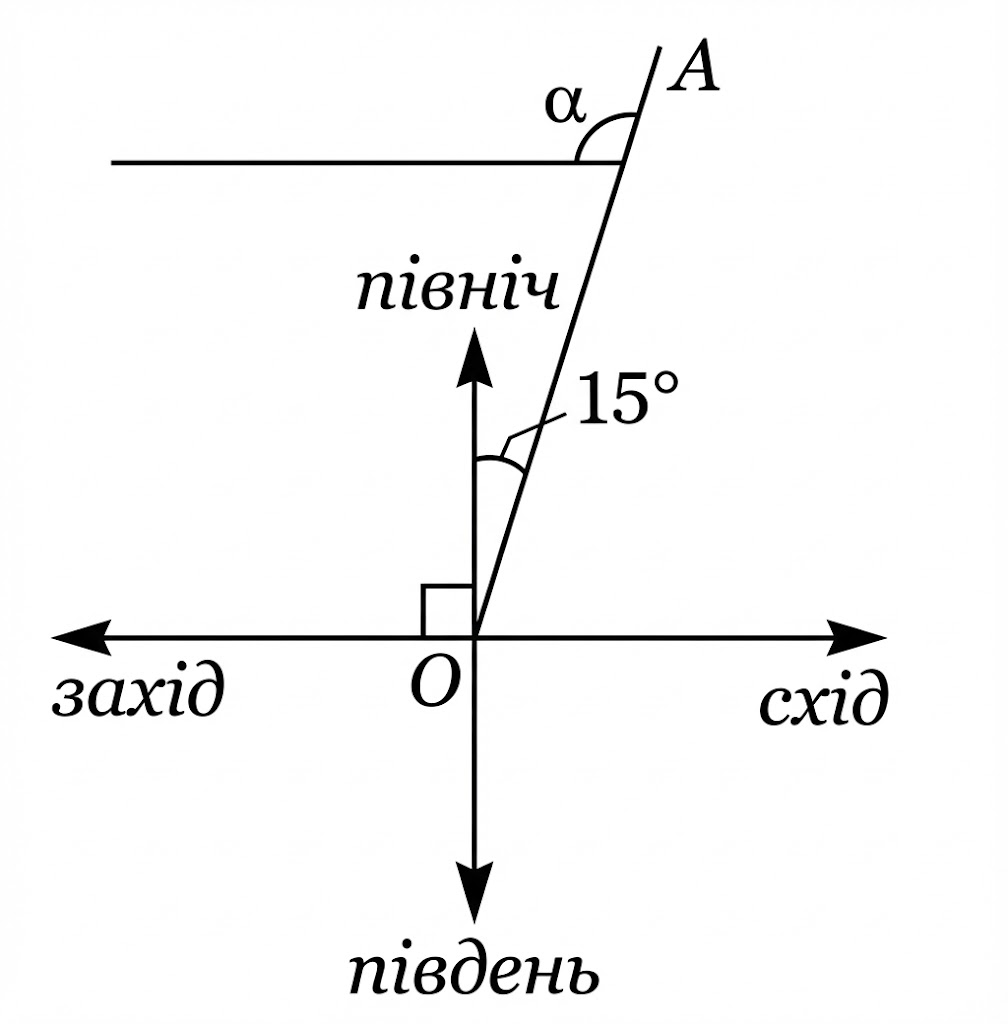
\includegraphics[scale=0.15]{tourists_compass.png}
\end{flushright}
\end{minipage}
\par\penalty-20\vspace{0.25cm}
\end{samepage}
\endgroup

\begingroup
% --- макроси, перенесені зі старого файлу теми ---
\providecommand{\matchingLayout}{}\renewcommand{\matchingLayout}[3]{
    \noindent
    \begin{minipage}[t]{0.36\textwidth}\vspace{0pt}\raggedright
       
        #1
    \end{minipage}%
    \hfill
    \begin{minipage}[t]{0.43\textwidth}\vspace{0pt}\raggedright
        
        #2
    \end{minipage}%
    \hfill
    \begin{minipage}[t]{0.19\textwidth}\vspace{0pt}\raggedright
        \vspace{0pt} % Хаки для вирівнювання minipage по верху
        \begin{flushright}
        #3
        \end{flushright}
    \end{minipage}
}

% --- сумісність зі старою базою (діє, якщо тема не має власного визначення) ---
\providecommand{\trigStyle}[1]{#1}
\providecommand{\answerTableSmall}[5]{%
\begingroup\setlength{\tabcolsep}{2pt}\small\nmtSetCell
\begin{tabular}{|*{5}{>{\centering\arraybackslash}m{\nmtcellw}|}}
\hline
\rule[-0.2cm]{0pt}{0.6cm}\textbf{А} & \textbf{Б} & \textbf{В} & \textbf{Г} & \textbf{Д} \\
\hline
\rule[-0.4cm]{0pt}{0.9cm}#1 & \rule[-0.4cm]{0pt}{0.9cm}#2 & \rule[-0.4cm]{0pt}{0.9cm}#3 & \rule[-0.4cm]{0pt}{0.9cm}#4 & \rule[-0.4cm]{0pt}{0.9cm}#5 \\
\hline
\end{tabular}\endgroup}
\providecommand{\matchingLayout}[3]{%
    \noindent
    \begin{minipage}[t]{0.36\textwidth}\vspace{0pt}\raggedright
        #1
    \end{minipage}%
    \hfill
    \begin{minipage}[t]{0.43\textwidth}\vspace{0pt}\raggedright
        #2
    \end{minipage}%
    \hfill
    \begin{minipage}[t]{0.19\textwidth}
        \vspace{0pt}
        \begin{flushright}
        #3
        \end{flushright}
    \end{minipage}}
\providecommand{\matchingLayoutBottom}[2]{%
    \noindent
    \begin{minipage}[t]{0.48\textwidth}\vspace{0pt}\raggedright
        #1
    \end{minipage}%
    \hfill
    \begin{minipage}[t]{0.48\textwidth}\vspace{0pt}\raggedright
        #2
    \end{minipage}
    \vspace{0.5cm}
    \noindent
    \matchingGrid}
\providecommand{\answerListVertical}[5]{%
    \par\nopagebreak\vspace{0.2cm}
    \begin{itemize}[itemsep=0.4cm, leftmargin=1.5cm, labelsep=0.5cm]
        \item[\textbf{А}] #1
        \item[\textbf{Б}] #2
        \item[\textbf{В}] #3
        \item[\textbf{Г}] #4
        \item[\textbf{Д}] #5
    \end{itemize}
    \vspace{0.2cm}}
\begin{samepage}
\noindent\zadnum Укажіть число, яке задовольняє систему нерівностей $\begin{cases} x > -3, \\ x \leqslant 7. \end{cases}$
\answerTable{$-3$}{$-10$}{$10$}{$5$}{$-6$}
\par\penalty-20
\end{samepage}
\endgroup

\begingroup
% --- макроси з файлів сесій НМТ-2026 (для рисунків) ---
\renewcommand{\headrulewidth}{0.4pt}
\renewcommand{\footrulewidth}{0.4pt}
\definecolor{gold}{RGB}{240, 190, 40}
\definecolor{silver}{RGB}{170, 170, 175}
\definecolor{bronze}{RGB}{190, 120, 70}
\definecolor{bar1}{RGB}{200, 120, 20}
\definecolor{bar2}{RGB}{255, 220, 0}
\definecolor{bar3}{RGB}{220, 30, 30}
\definecolor{bar4}{RGB}{128, 0, 128}
\definecolor{bar5}{RGB}{0, 160, 220}
\definecolor{bar6}{RGB}{120, 180, 50}

% --- сумісність зі старою базою (діє, якщо тема не має власного визначення) ---
\providecommand{\trigStyle}[1]{#1}
\providecommand{\answerTableSmall}[5]{%
\begingroup\setlength{\tabcolsep}{2pt}\small\nmtSetCell
\begin{tabular}{|*{5}{>{\centering\arraybackslash}m{\nmtcellw}|}}
\hline
\rule[-0.2cm]{0pt}{0.6cm}\textbf{А} & \textbf{Б} & \textbf{В} & \textbf{Г} & \textbf{Д} \\
\hline
\rule[-0.4cm]{0pt}{0.9cm}#1 & \rule[-0.4cm]{0pt}{0.9cm}#2 & \rule[-0.4cm]{0pt}{0.9cm}#3 & \rule[-0.4cm]{0pt}{0.9cm}#4 & \rule[-0.4cm]{0pt}{0.9cm}#5 \\
\hline
\end{tabular}\endgroup}
\providecommand{\matchingLayout}[3]{%
    \noindent
    \begin{minipage}[t]{0.36\textwidth}\vspace{0pt}\raggedright
        #1
    \end{minipage}%
    \hfill
    \begin{minipage}[t]{0.43\textwidth}\vspace{0pt}\raggedright
        #2
    \end{minipage}%
    \hfill
    \begin{minipage}[t]{0.19\textwidth}
        \vspace{0pt}
        \begin{flushright}
        #3
        \end{flushright}
    \end{minipage}}
\providecommand{\matchingLayoutBottom}[2]{%
    \noindent
    \begin{minipage}[t]{0.48\textwidth}\vspace{0pt}\raggedright
        #1
    \end{minipage}%
    \hfill
    \begin{minipage}[t]{0.48\textwidth}\vspace{0pt}\raggedright
        #2
    \end{minipage}
    \vspace{0.5cm}
    \noindent
    \matchingGrid}
\providecommand{\answerListVertical}[5]{%
    \par\nopagebreak\vspace{0.2cm}
    \begin{itemize}[itemsep=0.4cm, leftmargin=1.5cm, labelsep=0.5cm]
        \item[\textbf{А}] #1
        \item[\textbf{Б}] #2
        \item[\textbf{В}] #3
        \item[\textbf{Г}] #4
        \item[\textbf{Д}] #5
    \end{itemize}
    \vspace{0.2cm}}
\begin{samepage}
\noindent\zadnum Укажіть формулу для обчислення площі $S$ бічної поверхні циліндра, висота й радіус основи дорівнюють $R$.

\nmtnobreak
\nopagebreak\nbvspace{0.3cm}
\answerTableTall{$S=\pi R^2$}{$S=\dfrac{\pi R^2}{3}$}{$S=\dfrac{\pi R^3}{3}$}{$S=\pi R^3$}{$S=2\pi R^2$}
\par\penalty-20
\end{samepage}
\endgroup

\begin{samepage}
\zadtask{Спростіть вираз $\dfrac{12a^5 - 4a^5}{4}$.}
\answerTable{$2a^{10}$}{$2a^5$}{$12a^{10}$}{$-a^5$}{$11a^5$}
\par\penalty-20
\end{samepage}

\begingroup
% --- макроси, перенесені зі старого файлу теми ---
\providecommand{\matchingLayout}{}\renewcommand{\matchingLayout}[3]{
    \noindent
    \begin{minipage}[t]{0.36\textwidth}\vspace{0pt}\raggedright
       
        #1
    \end{minipage}%
    \hfill
    \begin{minipage}[t]{0.43\textwidth}\vspace{0pt}\raggedright
        
        #2
    \end{minipage}%
    \hfill
    \begin{minipage}[t]{0.19\textwidth}\vspace{0pt}\raggedright
        \vspace{0pt} % Хаки для вирівнювання minipage по верху
        \begin{flushright}
        #3
        \end{flushright}
    \end{minipage}
}

% --- сумісність зі старою базою (діє, якщо тема не має власного визначення) ---
\providecommand{\trigStyle}[1]{#1}
\providecommand{\answerTableSmall}[5]{%
\begingroup\setlength{\tabcolsep}{2pt}\small\nmtSetCell
\begin{tabular}{|*{5}{>{\centering\arraybackslash}m{\nmtcellw}|}}
\hline
\rule[-0.2cm]{0pt}{0.6cm}\textbf{А} & \textbf{Б} & \textbf{В} & \textbf{Г} & \textbf{Д} \\
\hline
\rule[-0.4cm]{0pt}{0.9cm}#1 & \rule[-0.4cm]{0pt}{0.9cm}#2 & \rule[-0.4cm]{0pt}{0.9cm}#3 & \rule[-0.4cm]{0pt}{0.9cm}#4 & \rule[-0.4cm]{0pt}{0.9cm}#5 \\
\hline
\end{tabular}\endgroup}
\providecommand{\matchingLayout}[3]{%
    \noindent
    \begin{minipage}[t]{0.36\textwidth}\vspace{0pt}\raggedright
        #1
    \end{minipage}%
    \hfill
    \begin{minipage}[t]{0.43\textwidth}\vspace{0pt}\raggedright
        #2
    \end{minipage}%
    \hfill
    \begin{minipage}[t]{0.19\textwidth}
        \vspace{0pt}
        \begin{flushright}
        #3
        \end{flushright}
    \end{minipage}}
\providecommand{\matchingLayoutBottom}[2]{%
    \noindent
    \begin{minipage}[t]{0.48\textwidth}\vspace{0pt}\raggedright
        #1
    \end{minipage}%
    \hfill
    \begin{minipage}[t]{0.48\textwidth}\vspace{0pt}\raggedright
        #2
    \end{minipage}
    \vspace{0.5cm}
    \noindent
    \matchingGrid}
\providecommand{\answerListVertical}[5]{%
    \par\nopagebreak\vspace{0.2cm}
    \begin{itemize}[itemsep=0.4cm, leftmargin=1.5cm, labelsep=0.5cm]
        \item[\textbf{А}] #1
        \item[\textbf{Б}] #2
        \item[\textbf{В}] #3
        \item[\textbf{Г}] #4
        \item[\textbf{Д}] #5
    \end{itemize}
    \vspace{0.2cm}}
\begin{samepage}
\zadtask{Позначте проміжок, якому належить корінь рівняння $\left(\dfrac{1}{3}\right)^{2x-1} = 9$.}
\answerTable{$(-3; -2)$}{$(-2; -1)$}{$(-1; 0)$}{$(0; 1)$}{$(1; 2)$}
\par\penalty-20
\end{samepage}
\endgroup

\begin{samepage}
\noindent
\begin{minipage}[c]{0.58\textwidth}
\zadnum Графік якої з наведених функцій зображено на рисунку?
\end{minipage}
\hfill
\begin{minipage}[c]{0.40\textwidth}
\centering
\begin{nmtfit}\begin{tikzpicture}[scale=0.7, thick]
    \draw[gray!35, very thin] (-2.5,-2.5) grid (4.5,2.5);
    \draw[->] (-2.8,0) -- (4.8,0) node[right] {\small $x$};
    \draw[->] (0,-2.8) -- (0,2.8) node[above] {\small $y$};
    \node[below right] at (0,0) {\scriptsize $0$};
    \node[below] at (1,0) {\scriptsize $1$};
    \node[left] at (0,1) {\scriptsize $1$};
    \draw[mainGreen, line width=1.2pt] (-2.3,1.3) -- (1,-2) -- (4.3,1.3);
\end{tikzpicture}\end{nmtfit}
\end{minipage}
\par\nbvspace{0.2cm}
\answerTable{$y = |x + 1| - 2$}{$y = |x - 1| - 2$}{$y = |x - 2| - 1$}{$y = -|x - 1| - 2$}{$y = |x - 1| + 2$}
\par\penalty-20
\end{samepage}

\begin{samepage}
\zadtask{Розгляньте наведені нижче твердження.\par
\nopagebreak\nbvspace{0.1cm}
\begin{enumerate}[label=\textbf{\Roman*.}, align=left, leftmargin=2.6em, labelsep=0.5em, itemsep=2pt, topsep=2pt]
\item Кожен кут рівностороннього трикутника дорівнює третині розгорнутого кута.
\item Кожен гострий кут тупокутного трикутника менший від $45^\circ$.
\item У прямокутному трикутнику хоча б один із гострих кутів не менший від $45^\circ$.
\end{enumerate}
\nopagebreak\nbvspace{0.1cm}
\noindent Які з тверджень є \textit{правильними}?}
\answerTable{лише I}{лише II}{лише I та II}{лише I та III}{I, II та III}
\par\penalty-20
\end{samepage}

\begingroup
% --- макроси, перенесені зі старого файлу теми ---
\definecolor{woodinner}{RGB}{222, 184, 135}
\definecolor{woodouter}{RGB}{139, 69, 19}

% --- сумісність зі старою базою (діє, якщо тема не має власного визначення) ---
\providecommand{\trigStyle}[1]{#1}
\providecommand{\answerTableSmall}[5]{%
\begingroup\setlength{\tabcolsep}{2pt}\small\nmtSetCell
\begin{tabular}{|*{5}{>{\centering\arraybackslash}m{\nmtcellw}|}}
\hline
\rule[-0.2cm]{0pt}{0.6cm}\textbf{А} & \textbf{Б} & \textbf{В} & \textbf{Г} & \textbf{Д} \\
\hline
\rule[-0.4cm]{0pt}{0.9cm}#1 & \rule[-0.4cm]{0pt}{0.9cm}#2 & \rule[-0.4cm]{0pt}{0.9cm}#3 & \rule[-0.4cm]{0pt}{0.9cm}#4 & \rule[-0.4cm]{0pt}{0.9cm}#5 \\
\hline
\end{tabular}\endgroup}
\providecommand{\matchingLayout}[3]{%
    \noindent
    \begin{minipage}[t]{0.36\textwidth}\vspace{0pt}\raggedright
        #1
    \end{minipage}%
    \hfill
    \begin{minipage}[t]{0.43\textwidth}\vspace{0pt}\raggedright
        #2
    \end{minipage}%
    \hfill
    \begin{minipage}[t]{0.19\textwidth}
        \vspace{0pt}
        \begin{flushright}
        #3
        \end{flushright}
    \end{minipage}}
\providecommand{\matchingLayoutBottom}[2]{%
    \noindent
    \begin{minipage}[t]{0.48\textwidth}\vspace{0pt}\raggedright
        #1
    \end{minipage}%
    \hfill
    \begin{minipage}[t]{0.48\textwidth}\vspace{0pt}\raggedright
        #2
    \end{minipage}
    \vspace{0.5cm}
    \noindent
    \matchingGrid}
\providecommand{\answerListVertical}[5]{%
    \par\nopagebreak\vspace{0.2cm}
    \begin{itemize}[itemsep=0.4cm, leftmargin=1.5cm, labelsep=0.5cm]
        \item[\textbf{А}] #1
        \item[\textbf{Б}] #2
        \item[\textbf{В}] #3
        \item[\textbf{Г}] #4
        \item[\textbf{Д}] #5
    \end{itemize}
    \vspace{0.2cm}}
\begin{samepage}
\zadtask{В арифметичній прогресії $(a_n)$ відомо, що $a_6 - a_1 = -30$. Знайдіть значення виразу $a_6 - a_4$.}
\answerTable{$-15$}{$-10$}{$10$}{$-12$}{$15$}
\par\penalty-20
\end{samepage}
\endgroup

\begingroup
% --- макроси з файлів сесій НМТ-2026 (для рисунків) ---
\renewcommand{\headrulewidth}{0.4pt}
\renewcommand{\footrulewidth}{0.4pt}
\definecolor{gold}{RGB}{240, 190, 40}
\definecolor{silver}{RGB}{170, 170, 175}
\definecolor{bronze}{RGB}{190, 120, 70}

% --- сумісність зі старою базою (діє, якщо тема не має власного визначення) ---
\providecommand{\trigStyle}[1]{#1}
\providecommand{\answerTableSmall}[5]{%
\begingroup\setlength{\tabcolsep}{2pt}\small\nmtSetCell
\begin{tabular}{|*{5}{>{\centering\arraybackslash}m{\nmtcellw}|}}
\hline
\rule[-0.2cm]{0pt}{0.6cm}\textbf{А} & \textbf{Б} & \textbf{В} & \textbf{Г} & \textbf{Д} \\
\hline
\rule[-0.4cm]{0pt}{0.9cm}#1 & \rule[-0.4cm]{0pt}{0.9cm}#2 & \rule[-0.4cm]{0pt}{0.9cm}#3 & \rule[-0.4cm]{0pt}{0.9cm}#4 & \rule[-0.4cm]{0pt}{0.9cm}#5 \\
\hline
\end{tabular}\endgroup}
\providecommand{\matchingLayout}[3]{%
    \noindent
    \begin{minipage}[t]{0.36\textwidth}\vspace{0pt}\raggedright
        #1
    \end{minipage}%
    \hfill
    \begin{minipage}[t]{0.43\textwidth}\vspace{0pt}\raggedright
        #2
    \end{minipage}%
    \hfill
    \begin{minipage}[t]{0.19\textwidth}
        \vspace{0pt}
        \begin{flushright}
        #3
        \end{flushright}
    \end{minipage}}
\providecommand{\matchingLayoutBottom}[2]{%
    \noindent
    \begin{minipage}[t]{0.48\textwidth}\vspace{0pt}\raggedright
        #1
    \end{minipage}%
    \hfill
    \begin{minipage}[t]{0.48\textwidth}\vspace{0pt}\raggedright
        #2
    \end{minipage}
    \vspace{0.5cm}
    \noindent
    \matchingGrid}
\providecommand{\answerListVertical}[5]{%
    \par\nopagebreak\vspace{0.2cm}
    \begin{itemize}[itemsep=0.4cm, leftmargin=1.5cm, labelsep=0.5cm]
        \item[\textbf{А}] #1
        \item[\textbf{Б}] #2
        \item[\textbf{В}] #3
        \item[\textbf{Г}] #4
        \item[\textbf{Д}] #5
    \end{itemize}
    \vspace{0.2cm}}
\begin{samepage}
\noindent\zadnum \begin{minipage}[t]{0.55\textwidth}
На дитячій каруселі розташовано 19 транспортних засобів: човники, літачки й машинки (див. рисунок). Дмитрик навмання сідає в один із транспортних засобів, \textit{окрім літачків}. Яка \textbf{ймовірність} того, що він сяде в \textit{машинку}?
\end{minipage}
\hfill
\begin{minipage}[t]{0.40\textwidth}
\nopagebreak\nbvspace{-0.3cm}
\begin{center}
\begin{nmtfit}\begin{tikzpicture}[scale=0.8]
    %
    \fill[yellow!10] (0,0) circle (4.0cm);
    \fill[cyan!10] (0,0) circle (3.2cm); %
    \fill[green!5] (0,0) circle (2.0cm); 

    %
    \draw[thick, gray!40] (0,0) circle (4.0cm);
    \draw[thick, gray!40] (0,0) circle (3.2cm);
    \draw[thick, gray!40] (0,0) circle (2.0cm);

    %
    \tikzset{icon/.style={thick, line join=round}}

    %
    \foreach \i in {1,...,10} {
        \pgfmathsetmacro{\ang}{\i * 360/10}
        \begin{scope}[rotate=\ang, shift={(3.5,0)}]
            \begin{scope}[rotate=90]
                 \draw[icon, fill=brown!80!black] (-0.35,0) arc (180:360:0.35 and 0.25) -- cycle;
                 \draw[icon, fill=white] (0,0.05) -- (0.25,0.05) -- (0,0.3) -- cycle; 
            \end{scope}
        \end{scope}
    }

    %
    \foreach \i in {1,...,5} {
        \pgfmathsetmacro{\ang}{\i * 360/5}
        \begin{scope}[rotate=\ang, shift={(2.6,0)}]
            \begin{scope}[rotate=90]
                \draw[icon, fill=cyan!80!blue] (-0.35,-0.2) rectangle (0.35,0.2);
                \draw[icon, fill=black] (-0.25,-0.2) circle (0.1); %
                \draw[icon, fill=black] (0.25,-0.2) circle (0.1);
                \draw[icon, fill=cyan!30] (-0.2,0) -- (-0.2,0.15) -- (0.2,0.15) -- (0.2,0) -- cycle; %
            \end{scope}
        \end{scope}
    }

    %
    \foreach \i in {1,...,4} {
        \pgfmathsetmacro{\ang}{\i * 360/4 + 45}
        \begin{scope}[rotate=\ang, shift={(1.2,0)}]
            \begin{scope}[rotate=90] 
                \draw[icon, fill=green!60!black] (0,-0.35) -- (0,0.4); %
                \draw[icon, fill=green!60!black] (-0.35,0) -- (0.35,0); %
                \draw[icon, fill=red] (-0.15,-0.3) -- (0.15,-0.3); %
            \end{scope}
        \end{scope}
    }

    %
    \node[anchor=west, font=\tiny] at (2.9, 3.5) {\textcolor{brown!80!black}{\rule{8pt}{8pt}} човник};
    \node[anchor=west, font=\tiny] at (2.9, 3.0) {\textcolor{green!60!black}{\rule{8pt}{8pt}} літачок};
    \node[anchor=west, font=\tiny] at (2.9, 2.5) {\textcolor{cyan!80!blue}{\rule{8pt}{8pt}} машинка};

\end{tikzpicture}\end{nmtfit}
\end{center}
\end{minipage}

\nmtnobreak
\nopagebreak\nbvspace{0.3cm}
\answerTableTall{$\dfrac{5}{19}$}{$\dfrac{1}{3}$}{$\dfrac{1}{15}$}{$\dfrac{2}{3}$}{$\dfrac{1}{5}$}
\par\penalty-20
\end{samepage}
\endgroup

\begingroup
% --- макроси, перенесені зі старого файлу теми ---
\providecommand{\matchingLayout}{}\renewcommand{\matchingLayout}[3]{
    \noindent
    \begin{minipage}[t]{0.36\textwidth}\vspace{0pt}\raggedright
       
        #1
    \end{minipage}%
    \hfill
    \begin{minipage}[t]{0.43\textwidth}\vspace{0pt}\raggedright
        
        #2
    \end{minipage}%
    \hfill
    \begin{minipage}[t]{0.19\textwidth}\vspace{0pt}\raggedright
        \vspace{0pt} % Хаки для вирівнювання minipage по верху
        \begin{flushright}
        #3
        \end{flushright}
    \end{minipage}
}

% --- макроси з файлів сесій НМТ-2026 (для рисунків) ---
\renewcommand{\headrulewidth}{0.4pt}
\renewcommand{\footrulewidth}{0.4pt}
\definecolor{hexcol}{RGB}{200,110,60}
\providecommand{\hexthree}{}\renewcommand{\hexthree}[2]{%
    \draw[hexcol, line width=1.1pt]
        ($(#1,#2)+(0:30)$) -- ($(#1,#2)+(60:30)$) -- ($(#1,#2)+(120:30)$) --
        ($(#1,#2)+(180:30)$) -- ($(#1,#2)+(240:30)$) -- ($(#1,#2)+(300:30)$) -- cycle;
}

% --- сумісність зі старою базою (діє, якщо тема не має власного визначення) ---
\providecommand{\trigStyle}[1]{#1}
\providecommand{\answerTableSmall}[5]{%
\begingroup\setlength{\tabcolsep}{2pt}\small\nmtSetCell
\begin{tabular}{|*{5}{>{\centering\arraybackslash}m{\nmtcellw}|}}
\hline
\rule[-0.2cm]{0pt}{0.6cm}\textbf{А} & \textbf{Б} & \textbf{В} & \textbf{Г} & \textbf{Д} \\
\hline
\rule[-0.4cm]{0pt}{0.9cm}#1 & \rule[-0.4cm]{0pt}{0.9cm}#2 & \rule[-0.4cm]{0pt}{0.9cm}#3 & \rule[-0.4cm]{0pt}{0.9cm}#4 & \rule[-0.4cm]{0pt}{0.9cm}#5 \\
\hline
\end{tabular}\endgroup}
\providecommand{\matchingLayout}[3]{%
    \noindent
    \begin{minipage}[t]{0.36\textwidth}\vspace{0pt}\raggedright
        #1
    \end{minipage}%
    \hfill
    \begin{minipage}[t]{0.43\textwidth}\vspace{0pt}\raggedright
        #2
    \end{minipage}%
    \hfill
    \begin{minipage}[t]{0.19\textwidth}
        \vspace{0pt}
        \begin{flushright}
        #3
        \end{flushright}
    \end{minipage}}
\providecommand{\matchingLayoutBottom}[2]{%
    \noindent
    \begin{minipage}[t]{0.48\textwidth}\vspace{0pt}\raggedright
        #1
    \end{minipage}%
    \hfill
    \begin{minipage}[t]{0.48\textwidth}\vspace{0pt}\raggedright
        #2
    \end{minipage}
    \vspace{0.5cm}
    \noindent
    \matchingGrid}
\providecommand{\answerListVertical}[5]{%
    \par\nopagebreak\vspace{0.2cm}
    \begin{itemize}[itemsep=0.4cm, leftmargin=1.5cm, labelsep=0.5cm]
        \item[\textbf{А}] #1
        \item[\textbf{Б}] #2
        \item[\textbf{В}] #3
        \item[\textbf{Г}] #4
        \item[\textbf{Д}] #5
    \end{itemize}
    \vspace{0.2cm}}
\begin{samepage}
\noindent\zadnum \begin{minipage}[t]{0.55\textwidth}
У прямокутній системі координат у просторі зображено прямокутний паралелепіпед, одна з вершин якого збігається з початком координат --- точкою $O$, а три ребра лежать на координатних осях (див. рисунок). Точка $K(12; 15; 16)$ є вершиною паралелепіпеда. Визначте довжину (модуль) вектора $\vec{OK}$.
\end{minipage}
\hfill
\begin{minipage}[t]{0.4\textwidth}
    \nopagebreak\nbvspace{-0.3cm}
    \begin{flushright}
    %
    \begin{nmtfit}\begin{tikzpicture}[x={(-0.5cm,-0.4cm)}, y={(0.8cm,0cm)}, z={(0cm,0.8cm)}, scale=0.15]

        %
        \coordinate (O) at (0,0,0);
        \coordinate (K) at (12,15,16);

        %
        \def\xk{12}
        \def\yk{15}
        \def\zk{16}

        %
        \coordinate (A) at (\xk,0,0);
        \coordinate (B) at (0,\yk,0);
        \coordinate (C) at (0,0,\zk);
        \coordinate (XY) at (\xk,\yk,0);
        \coordinate (XZ) at (\xk,0,\zk);
        \coordinate (YZ) at (0,\yk,\zk);

        %
        \draw[->, >=stealth] (0,0,0) -- (\xk+5,0,0) node[below left] {$x$};
        \draw[->, >=stealth] (0,0,0) -- (0,\yk+5,0) node[right] {$y$};
        \draw[->, >=stealth] (0,0,0) -- (0,0,\zk+5) node[left] {$z$};

        %
        \draw[dashed] (A) -- (XY) -- (B);
        \draw[dashed] (XY) -- (K);

        %
        \draw[thick] (O) -- (A) -- (XZ) -- (C) -- cycle; %
        \draw[thick] (O) -- (B) -- (YZ) -- (C) -- cycle; %
        %

        %
        %
        %

        %
        \draw[thick] (O) -- (A);
        \draw[thick] (O) -- (B);
        \draw[thick] (O) -- (C);

        \draw[thick] (A) -- (XZ);
        \draw[thick] (C) -- (XZ);
        \draw[thick] (C) -- (YZ);
        \draw[thick] (B) -- (YZ);
        \draw[thick] (XZ) -- (K);
        \draw[thick] (YZ) -- (K);

        %
        \draw[thick] (A) -- (XY) -- (B);
        \draw[thick] (XY) -- (K);

        %

        %
        \node[below right] at (O) {$O$};
        \node[above] at (K) {$K$};
        \fill (O) circle (8pt);
        \fill (K) circle (8pt);

    \end{tikzpicture}\end{nmtfit}
    \end{flushright}
\end{minipage}

\nmtnobreak
\nopagebreak\nbvspace{0.3cm}
\answerTable{$25$}{$43$}{$\sqrt{337}$}{$\sqrt{86}$}{$11$}
\par\penalty-20
\end{samepage}
\endgroup

\begingroup
% --- макроси, перенесені зі старого файлу теми ---
\providecommand{\matchingLayout}{}\renewcommand{\matchingLayout}[3]{
    \noindent
    \begin{minipage}[t]{0.36\textwidth}\vspace{0pt}\raggedright
       
        #1
    \end{minipage}%
    \hfill
    \begin{minipage}[t]{0.43\textwidth}\vspace{0pt}\raggedright
        
        #2
    \end{minipage}%
    \hfill
    \begin{minipage}[t]{0.19\textwidth}\vspace{0pt}\raggedright
        \vspace{0pt} % Хаки для вирівнювання minipage по верху
        \begin{flushright}
        #3
        \end{flushright}
    \end{minipage}
}
\providecommand{\trigStyle}{}\renewcommand{\trigStyle}[1]{\textbf{#1}}

% --- сумісність зі старою базою (діє, якщо тема не має власного визначення) ---
\providecommand{\trigStyle}[1]{#1}
\providecommand{\answerTableSmall}[5]{%
\begingroup\setlength{\tabcolsep}{2pt}\small\nmtSetCell
\begin{tabular}{|*{5}{>{\centering\arraybackslash}m{\nmtcellw}|}}
\hline
\rule[-0.2cm]{0pt}{0.6cm}\textbf{А} & \textbf{Б} & \textbf{В} & \textbf{Г} & \textbf{Д} \\
\hline
\rule[-0.4cm]{0pt}{0.9cm}#1 & \rule[-0.4cm]{0pt}{0.9cm}#2 & \rule[-0.4cm]{0pt}{0.9cm}#3 & \rule[-0.4cm]{0pt}{0.9cm}#4 & \rule[-0.4cm]{0pt}{0.9cm}#5 \\
\hline
\end{tabular}\endgroup}
\providecommand{\matchingLayout}[3]{%
    \noindent
    \begin{minipage}[t]{0.36\textwidth}\vspace{0pt}\raggedright
        #1
    \end{minipage}%
    \hfill
    \begin{minipage}[t]{0.43\textwidth}\vspace{0pt}\raggedright
        #2
    \end{minipage}%
    \hfill
    \begin{minipage}[t]{0.19\textwidth}
        \vspace{0pt}
        \begin{flushright}
        #3
        \end{flushright}
    \end{minipage}}
\providecommand{\matchingLayoutBottom}[2]{%
    \noindent
    \begin{minipage}[t]{0.48\textwidth}\vspace{0pt}\raggedright
        #1
    \end{minipage}%
    \hfill
    \begin{minipage}[t]{0.48\textwidth}\vspace{0pt}\raggedright
        #2
    \end{minipage}
    \vspace{0.5cm}
    \noindent
    \matchingGrid}
\providecommand{\answerListVertical}[5]{%
    \par\nopagebreak\vspace{0.2cm}
    \begin{itemize}[itemsep=0.4cm, leftmargin=1.5cm, labelsep=0.5cm]
        \item[\textbf{А}] #1
        \item[\textbf{Б}] #2
        \item[\textbf{В}] #3
        \item[\textbf{Г}] #4
        \item[\textbf{Д}] #5
    \end{itemize}
    \vspace{0.2cm}}
\begin{samepage}
\noindent\zadnum \trigStyle{$\dfrac{\cos(540^\circ - \alpha)}{\sin \alpha} = $}

\nmtnobreak
\nopagebreak\nbvspace{0.3cm}
\answerTableTall{$\dfrac{1}{\operatorname{tg} \alpha}$}{$-1$}{$1$}{$-\operatorname{tg} \alpha$}{$-\dfrac{1}{\operatorname{tg} \alpha}$}
\par\penalty-20
\end{samepage}
\endgroup

\begingroup
% --- макроси, перенесені зі старого файлу теми ---
\providecommand{\matchingLayout}{}\renewcommand{\matchingLayout}[3]{
    \noindent
    \begin{minipage}[t]{0.36\textwidth}\vspace{0pt}\raggedright
        #1
    \end{minipage}%
    \hfill
    \begin{minipage}[t]{0.43\textwidth}\vspace{0pt}\raggedright
        #2
    \end{minipage}%
    \hfill
    \begin{minipage}[t]{0.19\textwidth}\vspace{0pt}\raggedright
        \vspace{0pt} 
        \begin{flushright}
        #3
        \end{flushright}
    \end{minipage}
}

% --- макроси з файлів сесій НМТ-2026 (для рисунків) ---
\renewcommand{\headrulewidth}{0.4pt}
\renewcommand{\footrulewidth}{0.4pt}

% --- сумісність зі старою базою (діє, якщо тема не має власного визначення) ---
\providecommand{\trigStyle}[1]{#1}
\providecommand{\answerTableSmall}[5]{%
\begingroup\setlength{\tabcolsep}{2pt}\small\nmtSetCell
\begin{tabular}{|*{5}{>{\centering\arraybackslash}m{\nmtcellw}|}}
\hline
\rule[-0.2cm]{0pt}{0.6cm}\textbf{А} & \textbf{Б} & \textbf{В} & \textbf{Г} & \textbf{Д} \\
\hline
\rule[-0.4cm]{0pt}{0.9cm}#1 & \rule[-0.4cm]{0pt}{0.9cm}#2 & \rule[-0.4cm]{0pt}{0.9cm}#3 & \rule[-0.4cm]{0pt}{0.9cm}#4 & \rule[-0.4cm]{0pt}{0.9cm}#5 \\
\hline
\end{tabular}\endgroup}
\providecommand{\matchingLayout}[3]{%
    \noindent
    \begin{minipage}[t]{0.36\textwidth}\vspace{0pt}\raggedright
        #1
    \end{minipage}%
    \hfill
    \begin{minipage}[t]{0.43\textwidth}\vspace{0pt}\raggedright
        #2
    \end{minipage}%
    \hfill
    \begin{minipage}[t]{0.19\textwidth}
        \vspace{0pt}
        \begin{flushright}
        #3
        \end{flushright}
    \end{minipage}}
\providecommand{\matchingLayoutBottom}[2]{%
    \noindent
    \begin{minipage}[t]{0.48\textwidth}\vspace{0pt}\raggedright
        #1
    \end{minipage}%
    \hfill
    \begin{minipage}[t]{0.48\textwidth}\vspace{0pt}\raggedright
        #2
    \end{minipage}
    \vspace{0.5cm}
    \noindent
    \matchingGrid}
\providecommand{\answerListVertical}[5]{%
    \par\nopagebreak\vspace{0.2cm}
    \begin{itemize}[itemsep=0.4cm, leftmargin=1.5cm, labelsep=0.5cm]
        \item[\textbf{А}] #1
        \item[\textbf{Б}] #2
        \item[\textbf{В}] #3
        \item[\textbf{Г}] #4
        \item[\textbf{Д}] #5
    \end{itemize}
    \vspace{0.2cm}}
\begin{samepage}
\noindent\zadnum \begin{minipage}[t]{0.55\textwidth}
На сторонах $AD$ й $BC$ паралелограма $ABCD$ вибрано відповідно точки $K$ й $M$ так, що чотирикутник $KMCD$ є ромбом (див. рисунок). Визначте площу паралелограма $ABCD$, якщо $AK : KD = 1 : 2$, $KC = d$, $\angle CKD = \alpha$.
\end{minipage}
\hfill
\begin{minipage}[t]{0.4\textwidth}
    \nopagebreak\nbvspace{-0.3cm}
    \begin{flushright}
    \begin{nmtfit}\begin{tikzpicture}[scale=0.85]
        %
        \def\myAngle{25} 
        \def\sideKD{3} 

        \coordinate (K) at (0,0);
        \coordinate (D) at (\sideKD, 0);
        \coordinate (A) at (-1.5, 0); 

        %
        \coordinate (C) at ($(D) + ({2*\myAngle}:\sideKD)$);
        \coordinate (M) at ($(K) + ({2*\myAngle}:\sideKD)$);
        \coordinate (B) at ($(A) + ({2*\myAngle}:\sideKD)$);

        \draw[thick] (A) -- (B) -- (C) -- (D) -- cycle; 
        \draw[thick] (K) -- (M); 
        \draw[thick] (K) -- (C) node[midway, above left, xshift=2pt] {$d$}; 

        %
        \pic [draw, pic text={\small $\alpha$}, angle radius=0.9cm, angle eccentricity=1.2] {angle = D--K--C};

        \node[below left] at (A) {$A$};
        \node[above left] at (B) {$B$};
        \node[above right] at (C) {$C$};
        \node[below right] at (D) {$D$};
        \node[above] at (M) {$M$};
        \node[below] at (K) {$K$};

        \fill (K) circle (1.5pt);
        \fill (M) circle (1.5pt);
    \end{tikzpicture}\end{nmtfit}
    \end{flushright}
\end{minipage}

\nmtnobreak
\nopagebreak\nbvspace{0.2cm}
\answerTableTall{$\dfrac{3d^2\tg\alpha}{2}$}{$\dfrac{3d^2}{4\tg\alpha}$}{$\dfrac{3d^2\tg\alpha}{4}$}{$\dfrac{3d^2}{2\tg\alpha}$}{$\dfrac{4d^2\tg\alpha}{3}$}
\par\penalty-20
\end{samepage}
\endgroup

\begingroup
% --- сумісність зі старою базою (діє, якщо тема не має власного визначення) ---
\providecommand{\trigStyle}[1]{#1}
\providecommand{\answerTableSmall}[5]{%
\begingroup\setlength{\tabcolsep}{2pt}\small\nmtSetCell
\begin{tabular}{|*{5}{>{\centering\arraybackslash}m{\nmtcellw}|}}
\hline
\rule[-0.2cm]{0pt}{0.6cm}\textbf{А} & \textbf{Б} & \textbf{В} & \textbf{Г} & \textbf{Д} \\
\hline
\rule[-0.4cm]{0pt}{0.9cm}#1 & \rule[-0.4cm]{0pt}{0.9cm}#2 & \rule[-0.4cm]{0pt}{0.9cm}#3 & \rule[-0.4cm]{0pt}{0.9cm}#4 & \rule[-0.4cm]{0pt}{0.9cm}#5 \\
\hline
\end{tabular}\endgroup}
\providecommand{\matchingLayout}[3]{%
    \noindent
    \begin{minipage}[t]{0.36\textwidth}\vspace{0pt}\raggedright
        #1
    \end{minipage}%
    \hfill
    \begin{minipage}[t]{0.43\textwidth}\vspace{0pt}\raggedright
        #2
    \end{minipage}%
    \hfill
    \begin{minipage}[t]{0.19\textwidth}
        \vspace{0pt}
        \begin{flushright}
        #3
        \end{flushright}
    \end{minipage}}
\providecommand{\matchingLayoutBottom}[2]{%
    \noindent
    \begin{minipage}[t]{0.48\textwidth}\vspace{0pt}\raggedright
        #1
    \end{minipage}%
    \hfill
    \begin{minipage}[t]{0.48\textwidth}\vspace{0pt}\raggedright
        #2
    \end{minipage}
    \vspace{0.5cm}
    \noindent
    \matchingGrid}
\providecommand{\answerListVertical}[5]{%
    \par\nopagebreak\vspace{0.2cm}
    \begin{itemize}[itemsep=0.4cm, leftmargin=1.5cm, labelsep=0.5cm]
        \item[\textbf{А}] #1
        \item[\textbf{Б}] #2
        \item[\textbf{В}] #3
        \item[\textbf{Г}] #4
        \item[\textbf{Д}] #5
    \end{itemize}
    \vspace{0.2cm}}
\begin{samepage}
\zadtask{Розв'яжіть систему рівнянь $\begin{cases} \sqrt{y} - \dfrac{6}{x} = 6, \\[0.6cm] \sqrt{y} + \dfrac{4}{x} = 1. \end{cases}$ Якщо $(x_0; y_0)$ --- розв'язок системи, то $x_0 + y_0 =$}
\answerTable{$2$}{$9$}{$-2$}{$7$}{$83$}
\par\penalty-20
\end{samepage}
\endgroup

\instructionBox{У завданнях 16--18 до кожного з трьох рядків інформації, позначених цифрами, доберіть один правильний, на Вашу думку, варіант, позначений буквою.}

\begin{samepage}
\zadtask{Узгодьте вираз \mbox{(1--3)} із проміжком \mbox{(А--Д)}, якому належить значення цього виразу.
\par\nopagebreak\nbvspace{0.3cm}
\noindent
\matchingLayout{
\matchHead{Вираз}
\matchItem{1}{$\dfrac{4}{7} - \dfrac{3}{4}$}
\matchItem{2}{$\sqrt{0{,}5} \cdot \sqrt{32}$}
\matchItem{3}{$\log_8 4$}
}{
\matchHead{Проміжок}
\matchItem{А}{$[-1;\, 0)$}
\matchItem{Б}{$[0;\, 1)$}
\matchItem{В}{$[1;\, 2)$}
\matchItem{Г}{$[2;\, 4)$}
\matchItem{Д}{$[4;\, +\infty)$}
}{
\matchingGrid
}}
\par\penalty-20
\end{samepage}

\begin{samepage}
\zadtask{До кожного початку речення \mbox{(1--3)} доберіть його закінчення \mbox{(А--Д)} так, щоб утворилося правильне твердження.
\par\nopagebreak\nbvspace{0.3cm}
\noindent
\matchingLayout{
\matchHead{Початок речення}
\matchItem{1}{Графіки функцій $y = \dfrac{4}{x}$ та $y = -x$}
\matchItem{2}{Графіки функцій $y = \sqrt{x}$ та $y = x - 2$}
\matchItem{3}{Графік функції $y = x^2 - 2$ та графік рівняння $x^2 + y^2 = 4$}
}{
\matchHead{Закінчення речення}
\matchItem{А}{не мають спільних точок.}
\matchItem{Б}{мають єдину спільну точку.}
\matchItem{В}{мають лише дві спільні точки.}
\matchItem{Г}{мають лише три спільні точки.}
\matchItem{Д}{мають чотири спільні точки.}
}{
\matchingGrid
}}
\par\penalty-20
\end{samepage}

\begingroup
% --- макроси, перенесені зі старого файлу теми ---
\providecommand{\matchingLayout}{}\renewcommand{\matchingLayout}[3]{
    \noindent
    \begin{minipage}[t]{0.36\textwidth}\vspace{0pt}\raggedright
        #1
    \end{minipage}%
    \hfill
    \begin{minipage}[t]{0.43\textwidth}\vspace{0pt}\raggedright
        #2
    \end{minipage}%
    \hfill
    \begin{minipage}[t]{0.19\textwidth}\vspace{0pt}\raggedright
        \vspace{0pt} 
        \begin{flushright}
        #3
        \end{flushright}
    \end{minipage}
}

% --- макроси з файлів сесій НМТ-2026 (для рисунків) ---
\renewcommand{\headrulewidth}{0.4pt}
\renewcommand{\footrulewidth}{0.4pt}
\definecolor{gold}{RGB}{240, 190, 40}
\definecolor{silver}{RGB}{170, 170, 175}
\definecolor{bronze}{RGB}{190, 120, 70}
\definecolor{bar1}{RGB}{200, 120, 20}
\definecolor{bar2}{RGB}{255, 220, 0}
\definecolor{bar3}{RGB}{220, 30, 30}
\definecolor{bar4}{RGB}{128, 0, 128}
\definecolor{bar5}{RGB}{0, 160, 220}
\definecolor{bar6}{RGB}{120, 180, 50}

% --- сумісність зі старою базою (діє, якщо тема не має власного визначення) ---
\providecommand{\trigStyle}[1]{#1}
\providecommand{\answerTableSmall}[5]{%
\begingroup\setlength{\tabcolsep}{2pt}\small\nmtSetCell
\begin{tabular}{|*{5}{>{\centering\arraybackslash}m{\nmtcellw}|}}
\hline
\rule[-0.2cm]{0pt}{0.6cm}\textbf{А} & \textbf{Б} & \textbf{В} & \textbf{Г} & \textbf{Д} \\
\hline
\rule[-0.4cm]{0pt}{0.9cm}#1 & \rule[-0.4cm]{0pt}{0.9cm}#2 & \rule[-0.4cm]{0pt}{0.9cm}#3 & \rule[-0.4cm]{0pt}{0.9cm}#4 & \rule[-0.4cm]{0pt}{0.9cm}#5 \\
\hline
\end{tabular}\endgroup}
\providecommand{\matchingLayout}[3]{%
    \noindent
    \begin{minipage}[t]{0.36\textwidth}\vspace{0pt}\raggedright
        #1
    \end{minipage}%
    \hfill
    \begin{minipage}[t]{0.43\textwidth}\vspace{0pt}\raggedright
        #2
    \end{minipage}%
    \hfill
    \begin{minipage}[t]{0.19\textwidth}
        \vspace{0pt}
        \begin{flushright}
        #3
        \end{flushright}
    \end{minipage}}
\providecommand{\matchingLayoutBottom}[2]{%
    \noindent
    \begin{minipage}[t]{0.48\textwidth}\vspace{0pt}\raggedright
        #1
    \end{minipage}%
    \hfill
    \begin{minipage}[t]{0.48\textwidth}\vspace{0pt}\raggedright
        #2
    \end{minipage}
    \vspace{0.5cm}
    \noindent
    \matchingGrid}
\providecommand{\answerListVertical}[5]{%
    \par\nopagebreak\vspace{0.2cm}
    \begin{itemize}[itemsep=0.4cm, leftmargin=1.5cm, labelsep=0.5cm]
        \item[\textbf{А}] #1
        \item[\textbf{Б}] #2
        \item[\textbf{В}] #3
        \item[\textbf{Г}] #4
        \item[\textbf{Д}] #5
    \end{itemize}
    \vspace{0.2cm}}
\begin{samepage}
\zadtask{Вершини $A$ та $D$ прямокутника $ABCD$ є центрами кіл, які дотикаються ззовні, вершина $B$ належить більшому колу (див. рисунок). Радіуси більшого і меншого кіл дорівнюють $6$~см і $2$~см. Доберіть до відрізка \mbox{(1--3)} його довжину \mbox{(А--Д)}.\par
\nopagebreak\nbvspace{0.3cm}
\begin{center}
\begin{nmtfit}\begin{tikzpicture}[scale=0.42, thick, line join=round]
    \coordinate (A) at (0,0);
    \coordinate (B) at (0,6);
    \coordinate (C) at (8,6);
    \coordinate (D) at (8,0);
    \draw[gray!60] (A) circle (6);
    \draw[gray!60] (D) circle (2);
    \draw (A) -- (B) -- (C) -- (D) -- cycle;
    \fill (A) circle (4pt);
    \fill (D) circle (4pt);
    \fill (6,0) circle (3pt);
    \node[below left] at (A) {$A$};
    \node[above left] at (B) {$B$};
    \node[above right] at (C) {$C$};
    \node[below right, xshift=0.1cm] at (D) {$D$};
\end{tikzpicture}\end{nmtfit}
\end{center}
\nopagebreak\nbvspace{0.2cm}
\noindent
\matchingLayout{
\matchHead{Відрізок}
\matchItem{1}{$BC$}
\matchItem{2}{$BD$}
\matchItem{3}{відстань від точки $C$ до відрізка $BD$}
}{
\matchHead{Довжина відрізка}
\matchItem{А}{$4{,}8$~см}
\matchItem{Б}{$5$~см}
\matchItem{В}{$8$~см}
\matchItem{Г}{$10$~см}
\matchItem{Д}{$14$~см}
}{
\matchingGrid
}
}
\par\penalty-20
\end{samepage}
\endgroup

\instructionBox{Розв'яжіть завдання 19--22. Одержані числові відповіді запишіть у бланку відповідей. Відповідь записуйте лише десятковим дробом, урахувавши положення коми. Знак «мінус» записуйте перед першою цифрою числа.}

\begin{samepage}
\zadtask{Визначте критичні точки функції $f(x) = -4x^3 + 3x^2 + 36x - 11$. У відповідь запишіть ту з них, яка є \textit{точкою мінімуму}.}
\nmtAnswerBox
\par\penalty-20
\end{samepage}

\begingroup
% --- макроси з файлів сесій НМТ-2026 (для рисунків) ---
\definecolor{bar1}{RGB}{200, 120, 20}
\definecolor{bar2}{RGB}{255, 220, 0}
\definecolor{bar3}{RGB}{220, 30, 30}
\definecolor{bar4}{RGB}{128, 0, 128}
\definecolor{bar5}{RGB}{0, 160, 220}
\definecolor{bar6}{RGB}{120, 180, 50}
\renewcommand{\headrulewidth}{0.4pt}
\renewcommand{\footrulewidth}{0.4pt}

% --- сумісність зі старою базою (діє, якщо тема не має власного визначення) ---
\providecommand{\trigStyle}[1]{#1}
\providecommand{\answerTableSmall}[5]{%
\begingroup\setlength{\tabcolsep}{2pt}\small\nmtSetCell
\begin{tabular}{|*{5}{>{\centering\arraybackslash}m{\nmtcellw}|}}
\hline
\rule[-0.2cm]{0pt}{0.6cm}\textbf{А} & \textbf{Б} & \textbf{В} & \textbf{Г} & \textbf{Д} \\
\hline
\rule[-0.4cm]{0pt}{0.9cm}#1 & \rule[-0.4cm]{0pt}{0.9cm}#2 & \rule[-0.4cm]{0pt}{0.9cm}#3 & \rule[-0.4cm]{0pt}{0.9cm}#4 & \rule[-0.4cm]{0pt}{0.9cm}#5 \\
\hline
\end{tabular}\endgroup}
\providecommand{\matchingLayout}[3]{%
    \noindent
    \begin{minipage}[t]{0.36\textwidth}\vspace{0pt}\raggedright
        #1
    \end{minipage}%
    \hfill
    \begin{minipage}[t]{0.43\textwidth}\vspace{0pt}\raggedright
        #2
    \end{minipage}%
    \hfill
    \begin{minipage}[t]{0.19\textwidth}
        \vspace{0pt}
        \begin{flushright}
        #3
        \end{flushright}
    \end{minipage}}
\providecommand{\matchingLayoutBottom}[2]{%
    \noindent
    \begin{minipage}[t]{0.48\textwidth}\vspace{0pt}\raggedright
        #1
    \end{minipage}%
    \hfill
    \begin{minipage}[t]{0.48\textwidth}\vspace{0pt}\raggedright
        #2
    \end{minipage}
    \vspace{0.5cm}
    \noindent
    \matchingGrid}
\providecommand{\answerListVertical}[5]{%
    \par\nopagebreak\vspace{0.2cm}
    \begin{itemize}[itemsep=0.4cm, leftmargin=1.5cm, labelsep=0.5cm]
        \item[\textbf{А}] #1
        \item[\textbf{Б}] #2
        \item[\textbf{В}] #3
        \item[\textbf{Г}] #4
        \item[\textbf{Д}] #5
    \end{itemize}
    \vspace{0.2cm}}
\begin{samepage}
\noindent\zadnum У квітковому магазині є 12 білих і 25 червоних троянд. Покупець вибирає у цьому магазині дві білі й одну червону троянди. Скільки всього є варіантів такого вибору?

\nmtnobreak
\nopagebreak\nbvspace{0.5cm}
\nmtAnswerBox
\par\penalty-20
\end{samepage}
\endgroup

\begingroup
% --- макроси з файлів сесій НМТ-2026 (для рисунків) ---
\renewcommand{\headrulewidth}{0.4pt}
\renewcommand{\footrulewidth}{0.4pt}

% --- сумісність зі старою базою (діє, якщо тема не має власного визначення) ---
\providecommand{\trigStyle}[1]{#1}
\providecommand{\answerTableSmall}[5]{%
\begingroup\setlength{\tabcolsep}{2pt}\small\nmtSetCell
\begin{tabular}{|*{5}{>{\centering\arraybackslash}m{\nmtcellw}|}}
\hline
\rule[-0.2cm]{0pt}{0.6cm}\textbf{А} & \textbf{Б} & \textbf{В} & \textbf{Г} & \textbf{Д} \\
\hline
\rule[-0.4cm]{0pt}{0.9cm}#1 & \rule[-0.4cm]{0pt}{0.9cm}#2 & \rule[-0.4cm]{0pt}{0.9cm}#3 & \rule[-0.4cm]{0pt}{0.9cm}#4 & \rule[-0.4cm]{0pt}{0.9cm}#5 \\
\hline
\end{tabular}\endgroup}
\providecommand{\matchingLayout}[3]{%
    \noindent
    \begin{minipage}[t]{0.36\textwidth}\vspace{0pt}\raggedright
        #1
    \end{minipage}%
    \hfill
    \begin{minipage}[t]{0.43\textwidth}\vspace{0pt}\raggedright
        #2
    \end{minipage}%
    \hfill
    \begin{minipage}[t]{0.19\textwidth}
        \vspace{0pt}
        \begin{flushright}
        #3
        \end{flushright}
    \end{minipage}}
\providecommand{\matchingLayoutBottom}[2]{%
    \noindent
    \begin{minipage}[t]{0.48\textwidth}\vspace{0pt}\raggedright
        #1
    \end{minipage}%
    \hfill
    \begin{minipage}[t]{0.48\textwidth}\vspace{0pt}\raggedright
        #2
    \end{minipage}
    \vspace{0.5cm}
    \noindent
    \matchingGrid}
\providecommand{\answerListVertical}[5]{%
    \par\nopagebreak\vspace{0.2cm}
    \begin{itemize}[itemsep=0.4cm, leftmargin=1.5cm, labelsep=0.5cm]
        \item[\textbf{А}] #1
        \item[\textbf{Б}] #2
        \item[\textbf{В}] #3
        \item[\textbf{Г}] #4
        \item[\textbf{Д}] #5
    \end{itemize}
    \vspace{0.2cm}}
\begin{samepage}
\noindent\zadnum Задано сферу з площею поверхні $432\pi$~\text{см}$^2$ і правильну трикутну піраміду. Радіус кола, описаного навколо основи піраміди, дорівнює радіусу сфери, а висота піраміди – діаметру сфери. Визначте об’єм (у \text{см}$^3$) піраміди.

\nmtnobreak
\nopagebreak\nbvspace{0.5cm}
\nmtAnswerBox
\par\penalty-20
\end{samepage}
\endgroup

\begingroup
% --- сумісність зі старою базою (діє, якщо тема не має власного визначення) ---
\providecommand{\trigStyle}[1]{#1}
\providecommand{\answerTableSmall}[5]{%
\begingroup\setlength{\tabcolsep}{2pt}\small\nmtSetCell
\begin{tabular}{|*{5}{>{\centering\arraybackslash}m{\nmtcellw}|}}
\hline
\rule[-0.2cm]{0pt}{0.6cm}\textbf{А} & \textbf{Б} & \textbf{В} & \textbf{Г} & \textbf{Д} \\
\hline
\rule[-0.4cm]{0pt}{0.9cm}#1 & \rule[-0.4cm]{0pt}{0.9cm}#2 & \rule[-0.4cm]{0pt}{0.9cm}#3 & \rule[-0.4cm]{0pt}{0.9cm}#4 & \rule[-0.4cm]{0pt}{0.9cm}#5 \\
\hline
\end{tabular}\endgroup}
\providecommand{\matchingLayout}[3]{%
    \noindent
    \begin{minipage}[t]{0.36\textwidth}\vspace{0pt}\raggedright
        #1
    \end{minipage}%
    \hfill
    \begin{minipage}[t]{0.43\textwidth}\vspace{0pt}\raggedright
        #2
    \end{minipage}%
    \hfill
    \begin{minipage}[t]{0.19\textwidth}
        \vspace{0pt}
        \begin{flushright}
        #3
        \end{flushright}
    \end{minipage}}
\providecommand{\matchingLayoutBottom}[2]{%
    \noindent
    \begin{minipage}[t]{0.48\textwidth}\vspace{0pt}\raggedright
        #1
    \end{minipage}%
    \hfill
    \begin{minipage}[t]{0.48\textwidth}\vspace{0pt}\raggedright
        #2
    \end{minipage}
    \vspace{0.5cm}
    \noindent
    \matchingGrid}
\providecommand{\answerListVertical}[5]{%
    \par\nopagebreak\vspace{0.2cm}
    \begin{itemize}[itemsep=0.4cm, leftmargin=1.5cm, labelsep=0.5cm]
        \item[\textbf{А}] #1
        \item[\textbf{Б}] #2
        \item[\textbf{В}] #3
        \item[\textbf{Г}] #4
        \item[\textbf{Д}] #5
    \end{itemize}
    \vspace{0.2cm}}
\begin{samepage}
\noindent\zadnum Визначте \textit{додатне} значення параметра $m$, за якого один із коренів рівняння $x^2 - (2m - 2)x + 21 = 0$ на 4 більший від іншого.

\nmtnobreak
\nopagebreak\nbvspace{0.3cm}
\nmtAnswerBox
\par\penalty-20
\end{samepage}
\endgroup

\clearpage
\sectionTitle{Відповіді}

\begin{center}\small\renewcommand{\arraystretch}{1.25}
\begin{tabular}{|c|c|p{0.62\textwidth}|}\hline
\textbf{№} & \textbf{Відповідь} & \textbf{Джерело завдання} \\ \hline
1 & А & НМТ 2024, сесія 10.06.2024, № 3 \\ \hline
2 & А & НМТ 2026, сесія 15.06.2026, № 2 \\ \hline
3 & Г & НМТ 2024, сесія 14.06.2024, № 1 \\ \hline
4 & Г & НМТ 2025, сесія 02.06.2025, № 4 \\ \hline
5 & Д & НМТ 2023 \\ \hline
6 & Б & аналог (авторське завдання за зразком НМТ) \\ \hline
7 & В & НМТ 2026, сесія 10.06.2026, № 7 \\ \hline
8 & Б & аналог (авторське завдання за зразком НМТ) \\ \hline
9 & Г & аналог (авторське завдання за зразком НМТ) \\ \hline
10 & Г & НМТ 2024, сесія 04.06.2024, № 15 \\ \hline
11 & Б & НМТ 2025, сесія 11.06.2025, № 2 \\ \hline
12 & А & НМТ 2025, сесія 05.06.2025, № 10 \\ \hline
13 & Д & НМТ 2024 \\ \hline
14 & В & НМТ 2024, сесія 20.06.2024, № 12 \\ \hline
15 & Г & НМТ 2024, сесія 21.06.2024, № 15 \\ \hline
16 & 1~--~А, 2~--~Д, 3~--~Б & аналог (авторське завдання за зразком НМТ) \\ \hline
17 & 1~--~А, 2~--~Б, 3~--~Г & аналог (авторське завдання за зразком НМТ) \\ \hline
18 & 1~--~В, 2~--~Г, 3~--~А & НМТ 2026, сесія 11.06.2026, № 18 \\ \hline
19 & $-1{,}5$ & аналог (авторське завдання за зразком НМТ) \\ \hline
20 & $1650$ & НМТ 2023, сесія 08.06.2023, 1 зміна, № 17 \\ \hline
21 & $972$ & НМТ 2025, сесія 16.06.2025, № 22 \\ \hline
22 & $6$ & НМТ 2023 \\ \hline
\end{tabular}\end{center}

\noindent{\small\color{gray!80!black}Оцінювання: завдання 1--15 -- по 1 балу; 16--18 -- по 1 балу за кожну правильно встановлену відповідність (до 3 балів); 19--22 -- по 2 бали. Разом 32 бали.}

\end{document}
